% Important: If latex complains about unicode characters,
% please use "\usepackage[utf8x]{inputenc}" in your preamble
% You can change the size of the picture by putting it into the construct:
% 1) \resizebox{10cm}{!}{"below picture"} to scale horizontally to 10 cm
% 2) \resizebox{!}{15cm}{"below picture"} to scale vertically to 15 cm
% 3) \resizebox{10cm}{15cm}{"below picture"} a combination of above two
% It is not recomended to use the scale option of the tikzpicture environment.
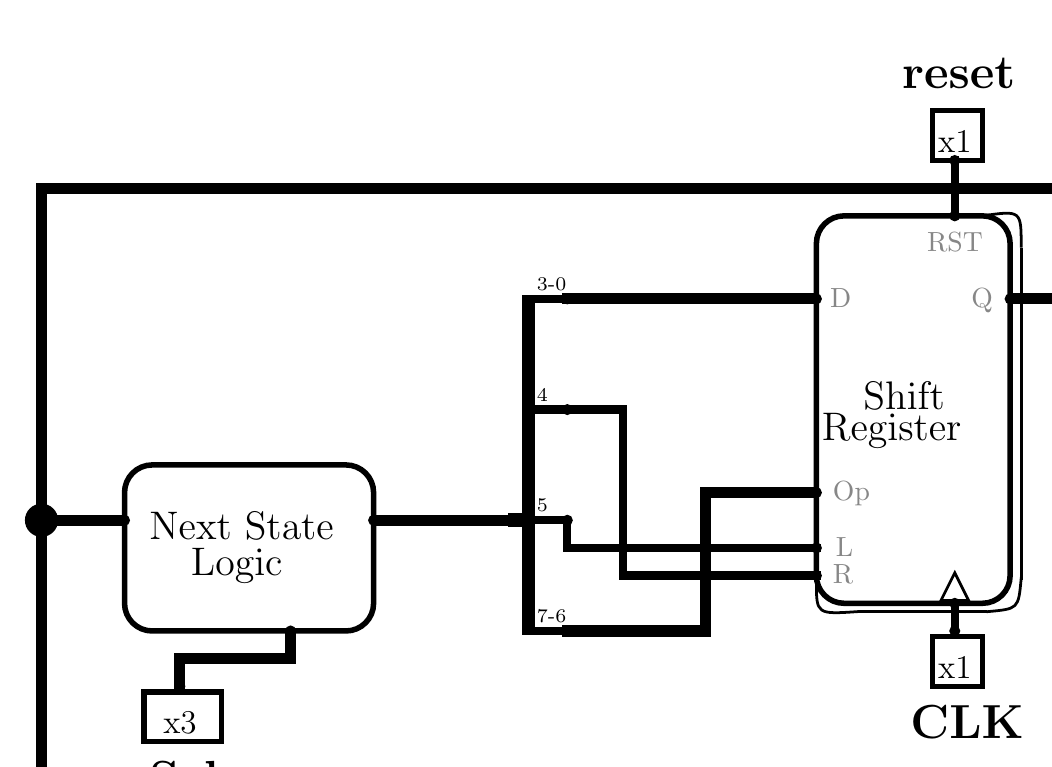
\begin{tikzpicture}[x=1pt,y=-1pt,line cap=rect]
\def\logisimfontA#1{\fontfamily{cmr}{#1}} % Replaced by logisim, original font was "SansSerif"
\def\logisimfontB#1{\fontfamily{Arial Rounded MT Bold}{#1}}
\definecolor{custcol_87_87_87}{RGB}{135, 135, 135}
\definecolor{custcol_0_0_0}{RGB}{0, 0, 0}
\definecolor{custcol_ff_ff_ff}{RGB}{255, 255, 255}
\draw [line width=3.0pt, custcol_0_0_0 ]  (335.0,208.0) -- (335.0,218.0) ;
\draw [line width=4.0pt, custcol_0_0_0 ]  (125.0,178.0) -- (175.0,178.0) ;
\draw [line width=3.0pt, custcol_0_0_0 ]  (335.0,48.0) -- (335.0,68.0) ;
\draw [line width=4.0pt, custcol_0_0_0 ]  (55.0,238.0) -- (55.0,228.0) -- (95.0,228.0) -- (95.0,218.0) ;
\draw [line width=4.0pt, custcol_0_0_0 ]  (35.0,178.0) -- (5.0,178.0) -- (5.0,308.0) -- (35.0,308.0) ;
\draw [line width=4.0pt, custcol_0_0_0 ]  (195.0,98.0) -- (285.0,98.0) ;
\draw [line width=4.0pt, custcol_0_0_0 ]  (105.0,358.0) -- (135.0,358.0) ;
\draw [line width=3.0pt, custcol_0_0_0 ]  (105.0,298.0) -- (135.0,298.0) ;
\draw [line width=4.0pt, custcol_0_0_0 ]  (105.0,318.0) -- (135.0,318.0) ;
\draw [line width=4.0pt, custcol_0_0_0 ]  (105.0,338.0) -- (135.0,338.0) ;
\draw [line width=3.0pt, custcol_0_0_0 ]  (105.0,378.0) -- (135.0,378.0) ;
\draw [line width=3.0pt, custcol_0_0_0 ]  (105.0,398.0) -- (135.0,398.0) ;
\draw [line width=4.0pt, custcol_0_0_0 ]  (105.0,418.0) -- (135.0,418.0) ;
\draw [line width=3.0pt, custcol_0_0_0 ]  (105.0,438.0) -- (135.0,438.0) ;
\draw [line width=3.0pt, custcol_0_0_0 ]  (105.0,458.0) -- (135.0,458.0) ;
\draw [line width=3.0pt, custcol_0_0_0 ]  (105.0,478.0) -- (135.0,478.0) ;
\draw [line width=3.0pt, custcol_0_0_0 ]  (105.0,498.0) -- (135.0,498.0) ;
\draw [line width=3.0pt, custcol_0_0_0 ]  (105.0,518.0) -- (135.0,518.0) ;
\draw [line width=3.0pt, custcol_0_0_0 ]  (105.0,538.0) -- (135.0,538.0) ;
\draw [line width=4.0pt, custcol_0_0_0 ]  (285.0,168.0) -- (245.0,168.0) -- (245.0,218.0) -- (195.0,218.0) ;
\draw [line width=4.0pt, custcol_0_0_0 ]  (355.0,98.0) -- (385.0,98.0) -- (385.0,58.0) -- (5.0,58.0) -- (5.0,178.0) ;
\fill [line width=3.0pt, custcol_0_0_0]  (5.0,178.0) ellipse (6.0 and 6.0 );
\draw [line width=2.0pt, custcol_0_0_0 ]  (42.0,240.0) -- (69.0,240.0) ;
\draw [line width=2.0pt, custcol_0_0_0 ]  (70.0,240.0) -- (70.0,257.0) ;
\draw [line width=2.0pt, custcol_0_0_0 ]  (70.0,258.0) -- (43.0,258.0) ;
\draw [line width=2.0pt, custcol_0_0_0 ]  (42.0,258.0) -- (42.0,241.0) ;
\logisimfontA{\fontsize{12pt}{12pt}\selectfont\node[inner sep=0, outer sep=0, custcol_0_0_0, anchor=base west] at  (49.0,255.0)  {x3};}
\logisimfontA{\fontsize{16pt}{16pt}\fontseries{bx}\selectfont\node[inner sep=0, outer sep=0, custcol_0_0_0, anchor=base west] at  (44.0,277.0)  {Sel};}
\fill [line width=2.0pt, custcol_0_0_0]  (55.0,238.0) ellipse (2.0 and 2.0 );
\draw [line width=2.0pt, custcol_0_0_0]  (146.0,299.0) ellipse (9.0 and 9.0 );
\logisimfontA{\fontsize{12pt}{12pt}\selectfont\node[inner sep=0, outer sep=0, custcol_0_0_0, anchor=base west] at  (139.0,305.0)  {x1};}
\logisimfontA{\fontsize{16pt}{16pt}\fontseries{bx}\selectfont\node[inner sep=0, outer sep=0, custcol_0_0_0, anchor=base west] at  (157.0,306.0)  {PCsrc};}
\fill [line width=2.0pt, custcol_0_0_0]  (135.0,298.0) ellipse (2.0 and 2.0 );
\begin{pgfpicture}
   \begin{pgfmagnify}{1pt}{-1pt}
      \pgfsetrectcap
      \pgfsetcornersarced{\pgfpoint{3.0}{3.0}}
      \pgfsetlinewidth{2.0}
      \color{custcol_0_0_0}
      \pgfsetfillopacity{1.0}
      \pgfpathrectanglecorners{\pgfpoint{137.0}{310.0}}{\pgfpoint{155.0}{328.0}}
      \pgfusepath{stroke}
   \end{pgfmagnify}
\end{pgfpicture}
\logisimfontA{\fontsize{12pt}{12pt}\selectfont\node[inner sep=0, outer sep=0, custcol_0_0_0, anchor=base west] at  (139.0,325.0)  {x2};}
\logisimfontA{\fontsize{16pt}{16pt}\fontseries{bx}\selectfont\node[inner sep=0, outer sep=0, custcol_0_0_0, anchor=base west] at  (157.0,326.0)  {ALUOp};}
\fill [line width=2.0pt, custcol_0_0_0]  (135.0,318.0) ellipse (2.0 and 2.0 );
\begin{pgfpicture}
   \begin{pgfmagnify}{1pt}{-1pt}
      \pgfsetrectcap
      \pgfsetcornersarced{\pgfpoint{3.0}{3.0}}
      \pgfsetlinewidth{2.0}
      \color{custcol_0_0_0}
      \pgfsetfillopacity{1.0}
      \pgfpathrectanglecorners{\pgfpoint{137.0}{330.0}}{\pgfpoint{155.0}{348.0}}
      \pgfusepath{stroke}
   \end{pgfmagnify}
\end{pgfpicture}
\logisimfontA{\fontsize{12pt}{12pt}\selectfont\node[inner sep=0, outer sep=0, custcol_0_0_0, anchor=base west] at  (139.0,345.0)  {x2};}
\logisimfontA{\fontsize{16pt}{16pt}\fontseries{bx}\selectfont\node[inner sep=0, outer sep=0, custcol_0_0_0, anchor=base west] at  (157.0,346.0)  {ALUsrcA};}
\fill [line width=2.0pt, custcol_0_0_0]  (135.0,338.0) ellipse (2.0 and 2.0 );
\begin{pgfpicture}
   \begin{pgfmagnify}{1pt}{-1pt}
      \pgfsetrectcap
      \pgfsetcornersarced{\pgfpoint{3.0}{3.0}}
      \pgfsetlinewidth{2.0}
      \color{custcol_0_0_0}
      \pgfsetfillopacity{1.0}
      \pgfpathrectanglecorners{\pgfpoint{137.0}{350.0}}{\pgfpoint{155.0}{368.0}}
      \pgfusepath{stroke}
   \end{pgfmagnify}
\end{pgfpicture}
\logisimfontA{\fontsize{12pt}{12pt}\selectfont\node[inner sep=0, outer sep=0, custcol_0_0_0, anchor=base west] at  (139.0,365.0)  {x2};}
\logisimfontA{\fontsize{16pt}{16pt}\fontseries{bx}\selectfont\node[inner sep=0, outer sep=0, custcol_0_0_0, anchor=base west] at  (157.0,366.0)  {ALUsrcB};}
\fill [line width=2.0pt, custcol_0_0_0]  (135.0,358.0) ellipse (2.0 and 2.0 );
\draw [line width=2.0pt, custcol_0_0_0]  (146.0,379.0) ellipse (9.0 and 9.0 );
\logisimfontA{\fontsize{12pt}{12pt}\selectfont\node[inner sep=0, outer sep=0, custcol_0_0_0, anchor=base west] at  (139.0,385.0)  {x1};}
\logisimfontA{\fontsize{16pt}{16pt}\fontseries{bx}\selectfont\node[inner sep=0, outer sep=0, custcol_0_0_0, anchor=base west] at  (157.0,386.0)  {PCbackWrite};}
\fill [line width=2.0pt, custcol_0_0_0]  (135.0,378.0) ellipse (2.0 and 2.0 );
\draw [line width=2.0pt, custcol_0_0_0]  (146.0,399.0) ellipse (9.0 and 9.0 );
\logisimfontA{\fontsize{12pt}{12pt}\selectfont\node[inner sep=0, outer sep=0, custcol_0_0_0, anchor=base west] at  (139.0,405.0)  {x1};}
\logisimfontA{\fontsize{16pt}{16pt}\fontseries{bx}\selectfont\node[inner sep=0, outer sep=0, custcol_0_0_0, anchor=base west] at  (157.0,406.0)  {RegWrite};}
\fill [line width=2.0pt, custcol_0_0_0]  (135.0,398.0) ellipse (2.0 and 2.0 );
\begin{pgfpicture}
   \begin{pgfmagnify}{1pt}{-1pt}
      \pgfsetrectcap
      \pgfsetcornersarced{\pgfpoint{3.0}{3.0}}
      \pgfsetlinewidth{2.0}
      \color{custcol_0_0_0}
      \pgfsetfillopacity{1.0}
      \pgfpathrectanglecorners{\pgfpoint{137.0}{410.0}}{\pgfpoint{155.0}{428.0}}
      \pgfusepath{stroke}
   \end{pgfmagnify}
\end{pgfpicture}
\logisimfontA{\fontsize{12pt}{12pt}\selectfont\node[inner sep=0, outer sep=0, custcol_0_0_0, anchor=base west] at  (139.0,425.0)  {x2};}
\logisimfontA{\fontsize{16pt}{16pt}\fontseries{bx}\selectfont\node[inner sep=0, outer sep=0, custcol_0_0_0, anchor=base west] at  (157.0,426.0)  {Mem2Reg};}
\fill [line width=2.0pt, custcol_0_0_0]  (135.0,418.0) ellipse (2.0 and 2.0 );
\draw [line width=2.0pt, custcol_0_0_0]  (146.0,439.0) ellipse (9.0 and 9.0 );
\logisimfontA{\fontsize{12pt}{12pt}\selectfont\node[inner sep=0, outer sep=0, custcol_0_0_0, anchor=base west] at  (139.0,445.0)  {x1};}
\logisimfontA{\fontsize{16pt}{16pt}\fontseries{bx}\selectfont\node[inner sep=0, outer sep=0, custcol_0_0_0, anchor=base west] at  (157.0,446.0)  {PCWriteCond};}
\fill [line width=2.0pt, custcol_0_0_0]  (135.0,438.0) ellipse (2.0 and 2.0 );
\draw [line width=2.0pt, custcol_0_0_0]  (146.0,459.0) ellipse (9.0 and 9.0 );
\logisimfontA{\fontsize{12pt}{12pt}\selectfont\node[inner sep=0, outer sep=0, custcol_0_0_0, anchor=base west] at  (139.0,465.0)  {x1};}
\logisimfontA{\fontsize{16pt}{16pt}\fontseries{bx}\selectfont\node[inner sep=0, outer sep=0, custcol_0_0_0, anchor=base west] at  (157.0,466.0)  {PCWrite};}
\fill [line width=2.0pt, custcol_0_0_0]  (135.0,458.0) ellipse (2.0 and 2.0 );
\draw [line width=2.0pt, custcol_0_0_0]  (146.0,479.0) ellipse (9.0 and 9.0 );
\logisimfontA{\fontsize{12pt}{12pt}\selectfont\node[inner sep=0, outer sep=0, custcol_0_0_0, anchor=base west] at  (139.0,485.0)  {x1};}
\logisimfontA{\fontsize{16pt}{16pt}\fontseries{bx}\selectfont\node[inner sep=0, outer sep=0, custcol_0_0_0, anchor=base west] at  (157.0,486.0)  {IorD};}
\fill [line width=2.0pt, custcol_0_0_0]  (135.0,478.0) ellipse (2.0 and 2.0 );
\draw [line width=2.0pt, custcol_0_0_0]  (146.0,499.0) ellipse (9.0 and 9.0 );
\logisimfontA{\fontsize{12pt}{12pt}\selectfont\node[inner sep=0, outer sep=0, custcol_0_0_0, anchor=base west] at  (139.0,505.0)  {x1};}
\logisimfontA{\fontsize{16pt}{16pt}\fontseries{bx}\selectfont\node[inner sep=0, outer sep=0, custcol_0_0_0, anchor=base west] at  (157.0,506.0)  {MemWrite};}
\fill [line width=2.0pt, custcol_0_0_0]  (135.0,498.0) ellipse (2.0 and 2.0 );
\draw [line width=2.0pt, custcol_0_0_0]  (146.0,519.0) ellipse (9.0 and 9.0 );
\logisimfontA{\fontsize{12pt}{12pt}\selectfont\node[inner sep=0, outer sep=0, custcol_0_0_0, anchor=base west] at  (139.0,525.0)  {x1};}
\logisimfontA{\fontsize{16pt}{16pt}\fontseries{bx}\selectfont\node[inner sep=0, outer sep=0, custcol_0_0_0, anchor=base west] at  (157.0,526.0)  {MemRead};}
\fill [line width=2.0pt, custcol_0_0_0]  (135.0,518.0) ellipse (2.0 and 2.0 );
\draw [line width=2.0pt, custcol_0_0_0]  (146.0,539.0) ellipse (9.0 and 9.0 );
\logisimfontA{\fontsize{12pt}{12pt}\selectfont\node[inner sep=0, outer sep=0, custcol_0_0_0, anchor=base west] at  (139.0,545.0)  {x1};}
\logisimfontA{\fontsize{16pt}{16pt}\fontseries{bx}\selectfont\node[inner sep=0, outer sep=0, custcol_0_0_0, anchor=base west] at  (157.0,546.0)  {IRWrite};}
\fill [line width=2.0pt, custcol_0_0_0]  (135.0,538.0) ellipse (2.0 and 2.0 );
\logisimfontB{\fontsize{10pt}{10pt}\selectfont\node[inner sep=0, outer sep=0, custcol_ff_ff_ff, anchor=base west] at  (147.0,486.0)  {OutLogic};}
\begin{pgfpicture}
   \begin{pgfmagnify}{1pt}{-1pt}
      \pgfsetrectcap
      \pgfsetcornersarced{\pgfpoint{10.0}{10.0}}
      \pgfsetlinewidth{1.0}
      \color{custcol_ff_ff_ff}
      \pgfsetfillopacity{1.0}
      \pgfpathrectanglecorners{\pgfpoint{35.0}{288.0}}{\pgfpoint{105.0}{548.0}}
      \pgfusepath{fill}
   \end{pgfmagnify}
\end{pgfpicture}
\begin{pgfpicture}
   \begin{pgfmagnify}{1pt}{-1pt}
      \pgfsetrectcap
      \pgfsetcornersarced{\pgfpoint{10.0}{10.0}}
      \pgfsetlinewidth{2.0}
      \color{custcol_0_0_0}
      \pgfsetfillopacity{1.0}
      \pgfpathrectanglecorners{\pgfpoint{35.0}{288.0}}{\pgfpoint{105.0}{548.0}}
      \pgfusepath{stroke}
   \end{pgfmagnify}
\end{pgfpicture}
\logisimfontB{\fontsize{16pt}{16pt}\selectfont\node[inner sep=0, outer sep=0, custcol_0_0_0, anchor=base west] at  (56.0,417.0)  {Out};}
\logisimfontB{\fontsize{16pt}{16pt}\selectfont\node[inner sep=0, outer sep=0, custcol_0_0_0, anchor=base west] at  (48.0,430.0)  {Logic};}
\fill [line width=1.0pt, custcol_0_0_0]  (35.0,308.0) ellipse (2.0 and 2.0 );
\fill [line width=1.0pt, custcol_0_0_0]  (105.0,298.0) ellipse (2.0 and 2.0 );
\fill [line width=1.0pt, custcol_0_0_0]  (105.0,318.0) ellipse (2.0 and 2.0 );
\fill [line width=1.0pt, custcol_0_0_0]  (105.0,338.0) ellipse (2.0 and 2.0 );
\fill [line width=1.0pt, custcol_0_0_0]  (105.0,358.0) ellipse (2.0 and 2.0 );
\fill [line width=1.0pt, custcol_0_0_0]  (105.0,378.0) ellipse (2.0 and 2.0 );
\fill [line width=1.0pt, custcol_0_0_0]  (105.0,398.0) ellipse (2.0 and 2.0 );
\fill [line width=1.0pt, custcol_0_0_0]  (105.0,418.0) ellipse (2.0 and 2.0 );
\fill [line width=1.0pt, custcol_0_0_0]  (105.0,438.0) ellipse (2.0 and 2.0 );
\fill [line width=1.0pt, custcol_0_0_0]  (105.0,458.0) ellipse (2.0 and 2.0 );
\fill [line width=1.0pt, custcol_0_0_0]  (105.0,478.0) ellipse (2.0 and 2.0 );
\fill [line width=1.0pt, custcol_0_0_0]  (105.0,498.0) ellipse (2.0 and 2.0 );
\fill [line width=1.0pt, custcol_0_0_0]  (105.0,518.0) ellipse (2.0 and 2.0 );
\fill [line width=1.0pt, custcol_0_0_0]  (105.0,538.0) ellipse (2.0 and 2.0 );
\begin{pgfpicture}
   \begin{pgfmagnify}{1pt}{-1pt}
      \pgfsetrectcap
      \pgfsetcornersarced{\pgfpoint{10.0}{10.0}}
      \pgfsetlinewidth{1.0}
      \color{custcol_ff_ff_ff}
      \pgfsetfillopacity{1.0}
      \pgfpathrectanglecorners{\pgfpoint{35.0}{158.0}}{\pgfpoint{125.0}{218.0}}
      \pgfusepath{fill}
   \end{pgfmagnify}
\end{pgfpicture}
\begin{pgfpicture}
   \begin{pgfmagnify}{1pt}{-1pt}
      \pgfsetrectcap
      \pgfsetcornersarced{\pgfpoint{10.0}{10.0}}
      \pgfsetlinewidth{2.0}
      \color{custcol_0_0_0}
      \pgfsetfillopacity{1.0}
      \pgfpathrectanglecorners{\pgfpoint{35.0}{158.0}}{\pgfpoint{125.0}{218.0}}
      \pgfusepath{stroke}
   \end{pgfmagnify}
\end{pgfpicture}
\logisimfontB{\fontsize{14pt}{14pt}\selectfont\node[inner sep=0, outer sep=0, custcol_0_0_0, anchor=base west] at  (44.0,185.0)  {Next State};}
\logisimfontB{\fontsize{14pt}{14pt}\selectfont\node[inner sep=0, outer sep=0, custcol_0_0_0, anchor=base west] at  (59.0,198.0)  {Logic};}
\fill [line width=1.0pt, custcol_0_0_0]  (35.0,178.0) ellipse (2.0 and 2.0 );
\fill [line width=1.0pt, custcol_0_0_0]  (95.0,218.0) ellipse (2.0 and 2.0 );
\fill [line width=1.0pt, custcol_0_0_0]  (125.0,178.0) ellipse (2.0 and 2.0 );
\begin{pgfpicture}
   \begin{pgfmagnify}{1pt}{-1pt}
      \pgfsetrectcap
      \pgfsetcornersarced{\pgfpoint{10.0}{10.0}}
      \pgfsetlinewidth{1.0}
      \color{custcol_ff_ff_ff}
      \pgfsetfillopacity{1.0}
      \pgfpathrectanglecorners{\pgfpoint{285.0}{68.0}}{\pgfpoint{355.0}{208.0}}
      \pgfusepath{fill}
   \end{pgfmagnify}
\end{pgfpicture}
\begin{pgfpicture}
   \begin{pgfmagnify}{1pt}{-1pt}
      \pgfsetrectcap
      \pgfsetcornersarced{\pgfpoint{10.0}{10.0}}
      \pgfsetlinewidth{2.0}
      \color{custcol_0_0_0}
      \pgfsetfillopacity{1.0}
      \pgfpathrectanglecorners{\pgfpoint{285.0}{68.0}}{\pgfpoint{355.0}{208.0}}
      \pgfusepath{stroke}
   \end{pgfmagnify}
\end{pgfpicture}
\logisimfontB{\fontsize{10pt}{10pt}\selectfont\node[inner sep=0, outer sep=0, custcol_87_87_87, anchor=base west] at  (325.0,81.0)  {RST};}
\logisimfontB{\fontsize{10pt}{10pt}\selectfont\node[inner sep=0, outer sep=0, custcol_87_87_87, anchor=base west] at  (292.0,191.0)  {L};}
\logisimfontB{\fontsize{10pt}{10pt}\selectfont\node[inner sep=0, outer sep=0, custcol_87_87_87, anchor=base west] at  (291.0,201.0)  {R};}
\logisimfontB{\fontsize{10pt}{10pt}\selectfont\node[inner sep=0, outer sep=0, custcol_87_87_87, anchor=base west] at  (290.0,101.0)  {D};}
\logisimfontB{\fontsize{10pt}{10pt}\selectfont\node[inner sep=0, outer sep=0, custcol_87_87_87, anchor=base west] at  (341.0,101.0)  {Q};}
\logisimfontB{\fontsize{10pt}{10pt}\selectfont\node[inner sep=0, outer sep=0, custcol_87_87_87, anchor=base west] at  (291.0,171.0)  {Op};}
\logisimfontB{\fontsize{14pt}{14pt}\fontseries{bx}\selectfont\node[inner sep=0, outer sep=0, custcol_0_0_0, anchor=base west] at  (302.0,138.0)  {Shift};}
\logisimfontB{\fontsize{14pt}{14pt}\fontseries{bx}\selectfont\node[inner sep=0, outer sep=0, custcol_0_0_0, anchor=base west] at  (287.0,149.0)  {Register};}
\draw [line width=1.0pt, custcol_0_0_0 ]  (359.0,79.0) .. controls  (359.0,66.0)  ..  (345.0,68.0) ;
\draw [line width=1.0pt, custcol_0_0_0 ]  (359.0,80.0) -- (359.0,199.0) ;
\draw [line width=1.0pt, custcol_0_0_0 ]  (347.0,211.0) .. controls  (358.0,210.0)  ..  (359.0,199.0) ;
\draw [line width=1.0pt, custcol_0_0_0 ]  (300.0,211.0) .. controls  (285.0,212.0)  ..  (285.0,200.0) ;
\draw [line width=1.0pt, custcol_0_0_0 ]  (301.0,211.0) -- (346.0,211.0) ;
\fill [line width=1.0pt, custcol_ff_ff_ff ]  (330.0,207.0) -- (335.0,197.0) -- (340.0,207.0) -- cycle;
\draw [line width=1.0pt, custcol_0_0_0 ]  (330.0,207.0) -- (335.0,197.0) -- (340.0,207.0) -- cycle;
\fill [line width=1.0pt, custcol_0_0_0]  (285.0,98.0) ellipse (2.0 and 2.0 );
\fill [line width=1.0pt, custcol_0_0_0]  (285.0,168.0) ellipse (2.0 and 2.0 );
\fill [line width=1.0pt, custcol_0_0_0]  (285.0,188.0) ellipse (2.0 and 2.0 );
\fill [line width=1.0pt, custcol_0_0_0]  (285.0,198.0) ellipse (2.0 and 2.0 );
\fill [line width=1.0pt, custcol_0_0_0]  (335.0,68.0) ellipse (2.0 and 2.0 );
\fill [line width=1.0pt, custcol_0_0_0]  (335.0,208.0) ellipse (2.0 and 2.0 );
\fill [line width=1.0pt, custcol_0_0_0]  (355.0,98.0) ellipse (2.0 and 2.0 );
\draw [line width=2.0pt, custcol_0_0_0 ]  (327.0,30.0) -- (344.0,30.0) ;
\draw [line width=2.0pt, custcol_0_0_0 ]  (345.0,30.0) -- (345.0,47.0) ;
\draw [line width=2.0pt, custcol_0_0_0 ]  (345.0,48.0) -- (328.0,48.0) ;
\draw [line width=2.0pt, custcol_0_0_0 ]  (327.0,48.0) -- (327.0,31.0) ;
\logisimfontA{\fontsize{12pt}{12pt}\selectfont\node[inner sep=0, outer sep=0, custcol_0_0_0, anchor=base west] at  (329.0,45.0)  {x1};}
\logisimfontA{\fontsize{16pt}{16pt}\fontseries{bx}\selectfont\node[inner sep=0, outer sep=0, custcol_0_0_0, anchor=base west] at  (316.0,22.0)  {reset};}
\fill [line width=2.0pt, custcol_0_0_0]  (335.0,48.0) ellipse (2.0 and 2.0 );
\draw [line width=3.0pt, custcol_0_0_0 ]  (195.0,98.0) -- (181.0,98.0) ;
\draw [line width=3.0pt, custcol_0_0_0 ]  (285.0,198.0) -- (215.0,198.0) -- (215.0,138.0) -- (195.0,138.0) -- (181.0,138.0) ;
\draw [line width=3.0pt, custcol_0_0_0 ]  (285.0,188.0) -- (195.0,188.0) -- (195.0,178.0) -- (181.0,178.0) ;
\draw [line width=3.0pt, custcol_0_0_0 ]  (195.0,218.0) -- (181.0,218.0) ;
\draw [line width=5.0pt, custcol_0_0_0 ]  (176.0,178.0) -- (181.0,178.0) ;
\draw [line width=5.0pt, custcol_0_0_0 ]  (181.0,99.0) -- (181.0,217.0) ;
\logisimfontA{\fontsize{7pt}{7pt}\selectfont\node[inner sep=0, outer sep=0, custcol_0_0_0, anchor=base west] at  (184.0,95.0)  {3-0};}
\logisimfontA{\fontsize{7pt}{7pt}\selectfont\node[inner sep=0, outer sep=0, custcol_0_0_0, anchor=base west] at  (184.0,135.0)  {4};}
\logisimfontA{\fontsize{7pt}{7pt}\selectfont\node[inner sep=0, outer sep=0, custcol_0_0_0, anchor=base west] at  (184.0,175.0)  {5};}
\logisimfontA{\fontsize{7pt}{7pt}\selectfont\node[inner sep=0, outer sep=0, custcol_0_0_0, anchor=base west] at  (184.0,215.0)  {7-6};}
\fill [line width=5.0pt, custcol_0_0_0]  (175.0,178.0) ellipse (2.0 and 2.0 );
\fill [line width=5.0pt, custcol_0_0_0]  (195.0,98.0) ellipse (2.0 and 2.0 );
\fill [line width=5.0pt, custcol_0_0_0]  (195.0,138.0) ellipse (2.0 and 2.0 );
\fill [line width=5.0pt, custcol_0_0_0]  (195.0,178.0) ellipse (2.0 and 2.0 );
\fill [line width=5.0pt, custcol_0_0_0]  (195.0,218.0) ellipse (2.0 and 2.0 );
\draw [line width=2.0pt, custcol_0_0_0 ]  (327.0,220.0) -- (344.0,220.0) ;
\draw [line width=2.0pt, custcol_0_0_0 ]  (345.0,220.0) -- (345.0,237.0) ;
\draw [line width=2.0pt, custcol_0_0_0 ]  (345.0,238.0) -- (328.0,238.0) ;
\draw [line width=2.0pt, custcol_0_0_0 ]  (327.0,238.0) -- (327.0,221.0) ;
\logisimfontA{\fontsize{12pt}{12pt}\selectfont\node[inner sep=0, outer sep=0, custcol_0_0_0, anchor=base west] at  (329.0,235.0)  {x1};}
\logisimfontA{\fontsize{16pt}{16pt}\fontseries{bx}\selectfont\node[inner sep=0, outer sep=0, custcol_0_0_0, anchor=base west] at  (319.0,257.0)  {CLK};}
\fill [line width=2.0pt, custcol_0_0_0]  (335.0,218.0) ellipse (2.0 and 2.0 );
\end{tikzpicture}

